

% \begin{table}
%     \centering
%     \label{tab:movielens_lfgcf_ablation}
%     \caption{数据集 MovieLens 下的 LFGCF 消融实验}
%     \begin{tabular}{ccc}
%         \toprule
%         \textbf{Model} & \textbf{Recall@10} &  \textbf{Recall@20} \\
%         \midrule
%         \begin{tabular}[c]{@{}c@{}}
%             LFGCF-L \\ LFGCF-T \\ LFGCF
%         \end{tabular} 
%         & \begin{tabular}[c]{@{}l@{}}
%             0.217 \\  0.2451\\ 0.25
%         \end{tabular}
%         & \begin{tabular}[c]{@{}l@{}}
%             0.2555  \\ 0.2903 \\  0.2939
%         \end{tabular} \\
%         \bottomrule
%     \end{tabular} 
% \end{table}

% \begin{table}
%     \centering
%     \label{tab:lastfm_lfgcf_ablation}
%     \caption{数据集 Last.FM 下的 LFGCF 消融实验}
%     \begin{tabular}{ccc}
%         \toprule
%         \textbf{Model} & \textbf{Recall@10} &  \textbf{Recall@20} \\
%         \midrule
%         \begin{tabular}[c]{@{}c@{}}
%             LFGCF-L \\ LFGCF-T \\ LFGCF
%         \end{tabular} 
%         & \begin{tabular}[c]{@{}l@{}}
%             0.4208 \\0.4336 \\ 0.4362 
%         \end{tabular}
%         & \begin{tabular}[c]{@{}l@{}}
%             0.4958 \\0.5027 \\ 0.5132
%         \end{tabular} \\
%         \bottomrule
%     \end{tabular} 
% \end{table}


% \begin{table}
%     \centering
%     \label{tab:delicious_lfgcf_ablation}
%     \caption{数据集 Delicious 下的 LFGCF 消融实验}
%     \begin{tabular}{ccc}
%         \toprule
%         \textbf{Model} & \textbf{Recall@10} &  \textbf{Recall@20} \\
%         \midrule
%         \begin{tabular}[c]{@{}c@{}}
%             LFGCF-L \\ LFGCF-T \\ LFGCF
%         \end{tabular} 
%         & \begin{tabular}[c]{@{}l@{}}
%             0.1615 \\ 0.1903 \\ 0.1955
%         \end{tabular}
%         & \begin{tabular}[c]{@{}l@{}}
%             0.2838 \\ 0.3270 \\ 0.3286
%         \end{tabular} \\
%         \bottomrule
%     \end{tabular} 
% \end{table}



% \begin{table}
%     \centering
%     % \label{tab:delicious_lfgcf_ablation}
%     \caption{数据集 MovieLens 下的 TAGCL 消融实验}
%     \begin{tabular}{ccc}
%         \toprule
%         \textbf{Model} & \textbf{Rec.@20} & \textbf{ARP.@20} \\
%         \midrule
%         \begin{tabular}[c]{@{}c@{}}
%             TAGCL-A \\ TAGCL-CL \\ TAGCL-NT \\ TAGCL-T  \\ TAGCL
%           \end{tabular} &
%           \begin{tabular}[c]{@{}c@{}} % recall
%             0.2883 \\ 0.3080 \\ 0.3169 \\ 0.3118 \\ \textbf{0.3180}
%           \end{tabular} & % ARP
%           \begin{tabular}[c]{@{}c@{}}
%             22.89 \\ 20.21 \\ 15.69 \\ 20.11 \\ \textbf{14.96}
%           \end{tabular} \\
%         \bottomrule
%     \end{tabular} 
% \end{table}

% \begin{table}
%     \centering
%     % \label{tab:delicious_lfgcf_ablation}
%     \caption{数据集 Last.FM 下的 TAGCL 消融实验}
%     \begin{tabular}{ccc}
%         \toprule
%         \textbf{Model} & \textbf{Rec.@20} & \textbf{ARP.@20} \\
%         \midrule
%         \begin{tabular}[c]{@{}c@{}}
%             TAGCL-A \\ TAGCL-CL \\ TAGCL-NT \\ TAGCL-T \\ TAGCL
%           \end{tabular} &
%           \begin{tabular}[c]{@{}c@{}} % recall
%             0.4502 \\ 0.4141 \\ \textbf{0.5212} \\ 0.5193 \\ 0.5199
%           \end{tabular} &
%           \begin{tabular}[c]{@{}c@{}} % ARP
%             92.05 \\ 89.42 \\ 43.92 \\ 52.17 \\ \textbf{42.99}
%           \end{tabular} \\
%         \bottomrule
%     \end{tabular} 
% \end{table}

% \begin{table}
%     \centering
%     % \label{tab:delicious_lfgcf_ablation}
%     \caption{数据集 Delicious 下的 TAGCL 消融实验}
%     \begin{tabular}{ccc}
%         \toprule
%         \textbf{Model} & \textbf{Rec.@20} & \textbf{ARP.@20} \\
%         \midrule
%         \begin{tabular}[c]{@{}c@{}}
%             TAGCL-A \\ TAGCL-CL \\ TAGCL-NT \\ TAGCL-T \\ TAGCL
%           \end{tabular} &
%           \begin{tabular}[c]{@{}c@{}} % recall
%             0.3188 \\ 0.3301 \\ 0.3425 \\ 0.3396 \\ \textbf{0.3432}
%           \end{tabular} &
%           \begin{tabular}[c]{@{}c@{}} % ndcg
%             5.33 \\ \textbf{5.24} \\ 5.48 \\ 5.58 \\ 5.61
%           \end{tabular} \\
%         \bottomrule
%     \end{tabular} 
% \end{table}


% \begin{figure*}[!h]
%     \centering
%     \begin{subfigure}{0.49\linewidth}
%         \centering
%         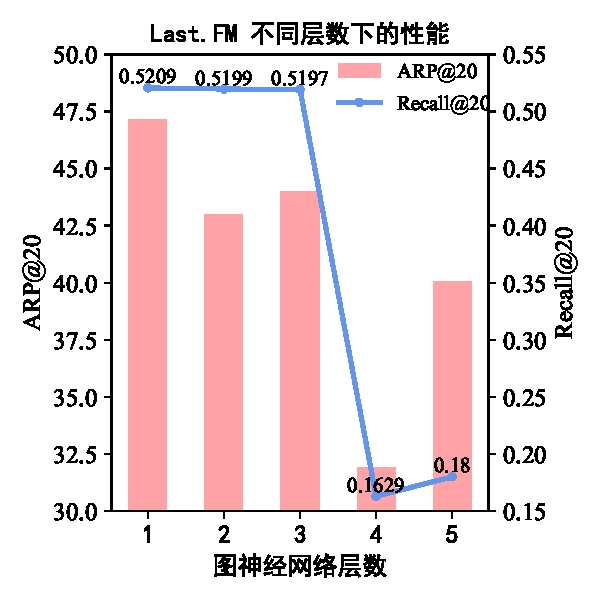
\includegraphics[width=.88\linewidth]{figure/tagcl_param_lastfm_layer.pdf}
%         \caption{layer}
%         \label{fig:tagcl_param_lastfm_layer}
%     \end{subfigure}
%     \begin{subfigure}{0.49\linewidth}
%         \centering
%         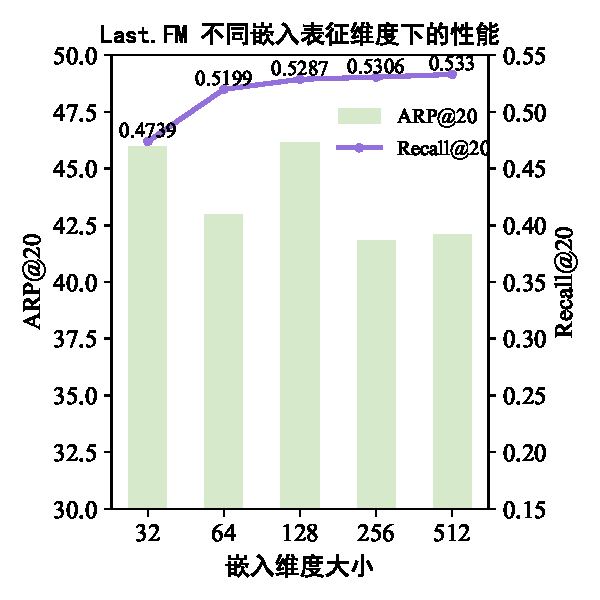
\includegraphics[width=.88\linewidth]{figure/tagcl_param_lastfm_emb.pdf}
%         \caption{emb}
%         \label{fig:tagcl_param_lastfm_emb}
%     \end{subfigure} 
%     \caption{Last.FM 下 TAGCL 的超参数实验}
%     \label{fig:lastfm_tagcl_param}
% \end{figure*}

% \begin{figure*}[!h]
%     \centering
%     \begin{subfigure}{0.49\linewidth}
%         \centering
%         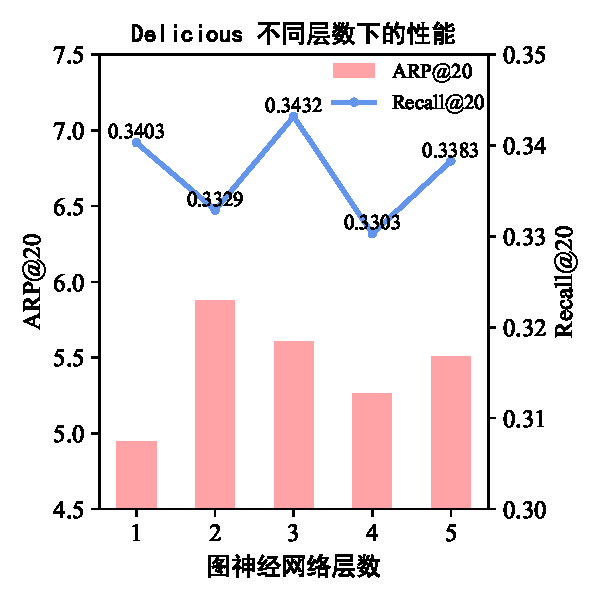
\includegraphics[width=.88\linewidth]{figure/tagcl_param_de_layer.pdf}
%         \caption{layer}
%         \label{fig:tagcl_param_de_layer}
%     \end{subfigure}
%     \begin{subfigure}{0.49\linewidth}
%         \centering
%         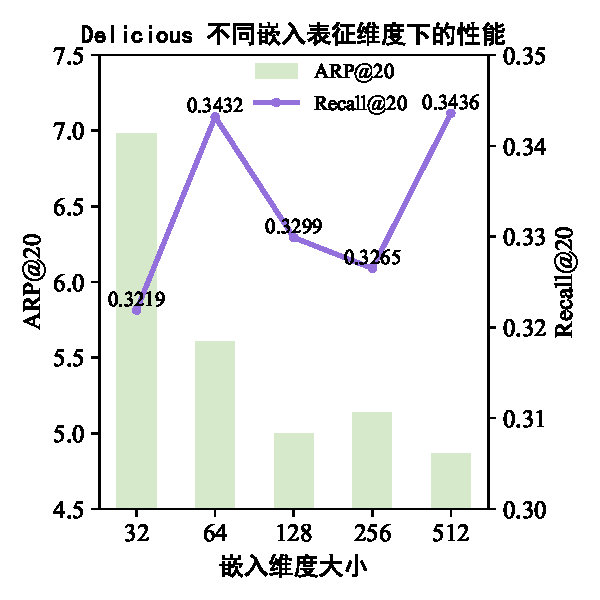
\includegraphics[width=.88\linewidth]{figure/tagcl_param_de_emb.pdf}
%         \caption{emb}
%         \label{fig:tagcl_param_de_emb}
%     \end{subfigure}
%     \caption{Last.FM 下 TAGCL 的超参数实验}
%     \label{fig:de_tagcl_param}
% \end{figure*}

\begin{table}
    \centering
      \caption{模型在 Delicious 上的复杂度}
      \label{tab:complexity}
      \begin{tabular}{c|cc|cc}
      \toprule
      \multirow{2}{*}{\textbf{模型}} &
      \multirow{2}{*}{\makecell[c]{参数量 \\ $(\times 10^6$)}} & 
      \multirow{2}{*}{\makecell[c]{相对 \\ 比率 (\%)}} &
      \multirow{2}{*}{\makecell[c]{推理 \\ 时间 (s)}} & 
      \multirow{2}{*}{\makecell[c]{相对 \\ 比率 (\%)}} \\
       & & & 
       \\
        \midrule
         \begin{tabular}[c]{@{}c@{}}
          LightGCN \\ NGCF  \\ LFGCF \\ GNN-PTR \\ TGCN 
          \end{tabular}
  
          & \begin{tabular}[c]{@{}l@{}}
            \textasciitilde4.33\\  \textasciitilde4.36 \\   \textasciitilde4.55 \\ \textasciitilde4.57 \\ \textasciitilde5.01 
            % 4359168
            % 4334208
            % 5018128
            % 4567104
            % 4558784
          \end{tabular}
          & \begin{tabular}[c]{@{}l@{}}
            -5.18\% \\ -4.58\%   \\ \makecell[c]{-} \\ +0.18\% \\ +9.15\% 
          \end{tabular} 
          & \begin{tabular}[c]{@{}l@{}}
            \textasciitilde0.14 \\ \textasciitilde0.15 \\ \textasciitilde0.13 \\ \textasciitilde0.17 \\ \textasciitilde2.12
          \end{tabular} 
          & \begin{tabular}[c]{@{}l@{}}
            +5.13\% \\ +13.91\% \\ \makecell[c]{-} \\ +16.33\% \\ +93.81\%
          \end{tabular} \\
        \bottomrule
      \end{tabular} 
  \end{table}

  % \begin{table}
  %   \centering
  %   \caption{TAGCL 在 BibSonomy 上的应用}
  %   \label{tab:bibsonomy}
  %   \begin{tabular}{cccccc}
  %     \toprule
  %     \multirow{2}{*}{\textbf{模型}} &
  %     \multicolumn{2}{c}{\textbf{BibSonomy-BM}} &
  %     \multicolumn{2}{c}{\textbf{BibSonomy-BT}} \\
  %     \cline{2-5} 
  %     & \textbf{Rec.@20} & \textbf{ARP.@20} & \textbf{Rec.@20} & \textbf{ARP.@20} \\
  %     \midrule
  %     LightGCN & 0.6117 & 1.53 & 0.4810 & 1.39 \\
  %     TAGCL & 0.6226 & 1.59 & 0.5173 & 1.67 \\
  %     \bottomrule
  %   \end{tabular}
  % \end{table}


  \begin{table}
    \centering
      \caption{模型在 Delicious 上的复杂度}
      \label{tab:complexity}
      \begin{tabular}{c|cc|cc}
      \toprule
      \multirow{2}{*}{\textbf{模型}} &
      \multirow{2}{*}{\makecell[c]{参数量 \\ $(\times 10^6$)}} & 
      \multirow{2}{*}{\makecell[c]{相对 \\ 比率 (\%)}} &
      \multirow{2}{*}{\makecell[c]{推理 \\ 时间 (s)}} & 
      \multirow{2}{*}{\makecell[c]{相对 \\ 比率 (\%)}} \\
       & & & 
       \\
        \midrule
         \begin{tabular}[c]{@{}c@{}}
          LightGCN \\ NGCF  \\ LFGCF \\ GNN-PTR \\ TGCN 
          \end{tabular}
  
          & \begin{tabular}[c]{@{}l@{}}
            \textasciitilde4.33\\  \textasciitilde4.36 \\   \textasciitilde4.55 \\ \textasciitilde4.57 \\ \textasciitilde5.01 
            % 4359168
            % 4334208
            % 5018128
            % 4567104
            % 4558784
          \end{tabular}
          & \begin{tabular}[c]{@{}l@{}}
            -5.18\% \\ -4.58\%   \\ \makecell[c]{-} \\ +0.18\% \\ +9.15\% 
          \end{tabular} 
          & \begin{tabular}[c]{@{}l@{}}
            \textasciitilde0.14 \\ \textasciitilde0.15 \\ \textasciitilde0.13 \\ \textasciitilde0.17 \\ \textasciitilde2.12
          \end{tabular} 
          & \begin{tabular}[c]{@{}l@{}}
            +5.13\% \\ +13.91\% \\ \makecell[c]{-} \\ +16.33\% \\ +93.81\%
          \end{tabular} \\
        \bottomrule
      \end{tabular} 
  \end{table}


  